\begin{align}
 & \norm{\vec{A}-\vec{B}}  =    \norm{\vec{B}-\vec{A}} \\
 & (\vec{B}-\vec{A})^T(\vec{B}-\vec{C})  =  \norm{\vec{A}-\vec{B}}^2 - (\vec{A}-\vec{C})^T(\vec{A}-\vec{B}) 
\end{align}
\begin{figure}[!htb]
	\centering
	\centering
	\resizebox{\columnwidth}{!}{%\documentclass{article}
%\usepackage[utf8]{inputenc}
%\usepackage{tikz}
%\usetikzlibrary{positioning}

%\begin{document}
	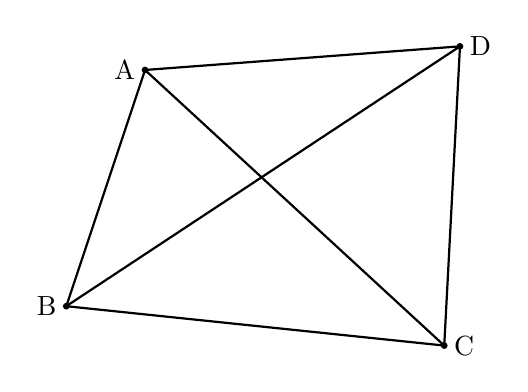
\begin{tikzpicture}
		\draw[black, thick] (0,0) --(1.0001,3); 
		\filldraw[black] (0,0) circle (1pt) node[anchor=east] {B}; 
		\draw[black, thick] (1.0001,3)--(5,3.3);
		\filldraw[black] (1.0001,3) circle (1pt) node[anchor=east] {A};
		\draw[black, thick] (5,3.3)--(4.8,-0.5);
		\filldraw[black] (5,3.3) circle (1pt) node[anchor=west] {D};
		\draw[black, thick] (4.8,-0.5)--(0,0);
		\filldraw[black] (4.8,-0.5) circle (1pt) node[anchor=west] {C};
		\draw[black, thick] (5,3.3)--(0,0);
		\draw[black, thick] (1.0001,3)--(4.8,-0.5);
	\end{tikzpicture}


%\end{document}}
	\caption{Quadrilateral ABCD with AD = BC and $\angle$ DAB = $\angle$CBA}
\end{figure}
ABCD is a quadrilateral, where AD=BC and $\angle DAB= \angle CBA$.

To show $\triangle ABD \cong \triangle BAC$, we use
\begin{align}
	& \angle DAB = \angle CBA & (Given) \\
	& AD = BC & (Given) \\
	& AB = BA & (Common \enspace Side)
\end{align}
Thus, by SAS Congruency Criteria, $\triangle ABD \cong \triangle BAC$.

Also, we are given that
\begin{align}
 & \angle DAB  =  \angle CBA \\
 \implies &\cos\angle DAB  =  \cos\angle CBA \\
 &  \frac{(\vec A -\vec B)^T(\vec{A}-\vec{D})}{\norm{\vec{A}-\vec{B}} \norm{\vec{A}-\vec{D}} } = \frac{(\vec B -\vec A)^T(\vec{B}-\vec{C})}{\norm{\vec{B}-\vec{A}} \norm{\vec{B}-\vec{C}}}
 \end{align}
Since,
\begin{align}
	& \norm{\vec{A}-\vec{D}}  =  \norm{\vec{B}-\vec{C}} \\
	\implies & \frac{(\vec A -\vec B)^T(\vec{A}-\vec{D})}{\norm{\vec{A}-\vec{B}}} = \frac{(\vec B -\vec A)^T(\vec{B}-\vec{C})}{\norm{\vec{B}-\vec{A}}} \\
    \implies & (\vec A -\vec B)^T(\vec{A}-\vec{D}) =  (\vec B -\vec A)^T(\vec{B}-\vec{C})
\end{align}
\begin{multline}
 \implies \norm{\vec{A}-\vec{B}}^2 - (\vec B -\vec A)^T(\vec{B}-\vec{D})  =\\ \norm{\vec{A}-\vec{B}}^2 - (\vec A -\vec B)^T(\vec{A}-\vec{C}) 
\end{multline}
\begin{align}
& (\vec B -\vec A)^T(\vec{B}-\vec{D}) = (\vec A -\vec B)^T(\vec{A}-\vec{C})\label{1}
\end{align}
\begin{multline}
 \norm{\vec{B} - \vec{A}}\norm{\vec{B} - \vec{D}}\cos\angle ABD  = \\ \norm{\vec{A} - \vec{B}}\norm{\vec{A} - \vec{C}}\cos\angle BAC 	
\end{multline}
\begin{align}
 \norm{\vec{B} - \vec{D}}\cos\angle ABD  = \norm{\vec{A} - \vec{C}}\cos\angle BAC \label{2}
\end{align}
\begin{enumerate}
\item To Prove $\norm{\vec{B} - \vec{D}} = \norm{\vec{A} - \vec{C}}$. 

From \eqref{1},
\begin{align}
	& (\vec B -\vec A)^T(\vec{B}-\vec{D}) = (\vec A -\vec B)^T(\vec{A}-\vec{C})
\end{align}
\begin{multline}
\norm{\vec{B}-\vec{D}}^2 - (\vec D -\vec B)^T(\vec{D}-\vec{A})= \\ \norm{\vec{A}-\vec{C}}^2 - (\vec C -\vec B)^T(\vec{C}-\vec{A})	
\end{multline}
\begin{multline}
 \norm{\vec{B}-\vec{D}}^2 - (\norm{\vec{A}-\vec{D}}^2 - (\vec A -\vec B)^T(\vec A -\vec D))   = \\
 \norm{\vec{A}-\vec{C}}^2 - (\norm{\vec{B}-\vec{C}}^2 - (\vec B -\vec A)^T(\vec B -\vec C))\	
\end{multline}
We know that
\begin{align}
	\norm{\vec{A}-\vec{D}} =  \norm{\vec{B}-\vec{C}} 
\end{align}
\begin{multline}
\norm{\vec{B}-\vec{D}}^2 + (\vec A -\vec B)^T(\vec{A}-\vec{D}) = \\ \norm{\vec{A}-\vec{C}}^2 + (\vec B -\vec A)^T(\vec{B}-\vec{C}) 	
\end{multline}
\begin{multline}
\norm{\vec{B}-\vec{D}}^2 + \norm{\vec{A}-\vec{B}}\norm{\vec{A}-\vec{D}}\cos \angle DAB = \\
 \norm{\vec{A}-\vec{C}}^2 + \norm{\vec{B}-\vec{A}}\norm{\vec{B}-\vec{C}}\cos \angle CBA \label{3}	
\end{multline}
Since, we are given that $\angle DAB = \angle CBA$ and $\norm{\vec{A}-\vec{D}} = \norm{\vec{B}-\vec{C}}$. Then by \eqref{3}
\begin{align}
	& \norm{\vec{B}-\vec{D}}^2 = \norm{\vec{A}-\vec{C}}^2 \\
	& \label{4}\norm{\vec{B}-\vec{D}} = \norm{\vec{A}-\vec{C}}
\end{align}
Hence, BD = AC.
\end{enumerate}
